\documentclass[11pt]{article}

\usepackage[margin=1in]{geometry}
\usepackage{amsmath, amssymb}
\usepackage{booktabs}
\usepackage{graphicx}
\usepackage{hyperref}

\graphicspath{
    {../outputs/plots/}
    {../outputs/plots/details/interior/}
}

\title{Guide to the Seller A Best-Response Plots}
\author{}
\date{}

\begin{document}
\maketitle

\section{Model Objects Used in the Plots}

The state in the simulation is the user's history with Seller A,
\[
    (S,F),
\]
where $S$ is the number of successes previously observed from Seller A and $F$
is the number of failures. Because the user does not observe Seller A's hidden
product choice, the user updates a misspecified single-product belief,
\[
    \theta \mid S,F \sim \operatorname{Beta}(1+S,1+F).
\]
The probability that the Thompson-sampling user chooses Seller A is
\[
    \rho(S,F)
    =
    \Pr(\tilde{\theta} \ge p_0 \mid S,F),
    \qquad
    \tilde{\theta} \sim \operatorname{Beta}(1+S,1+F),
\]
where $p_0$ is the known success probability of Seller B.

For product $x \in \{1,2\}$, define Seller A's product-specific action value as
\[
    Q_x(S,F)
    =
    R-c_x
    +
    \gamma \left[
        p_x V(S+1,F)
        +
        (1-p_x)V(S,F+1)
    \right].
\]
The optimal product at state $(S,F)$ is the product with the larger $Q$ value.
Equivalently, product 2 is optimal when
\[
    Q_2(S,F) - Q_1(S,F) \ge 0.
\]
Since
\[
    Q_2(S,F)-Q_1(S,F)
    =
    -(c_2-c_1)
    +
    (p_2-p_1)M_t(S,F),
\]
where
\[
    M_t(S,F)
    =
    \gamma\left[V_{t+1}(S+1,F)-V_{t+1}(S,F+1)\right],
\]
product 2 is optimal exactly when
\[
    M_t(S,F)
    \ge
    \frac{c_2-c_1}{p_2-p_1}
    =
    \frac{4}{3}.
\]
If the undiscounted raw difference
$D_t=V_{t+1}(S+1,F)-V_{t+1}(S,F+1)$ is reported instead, its threshold is
$(c_2-c_1)/[\gamma(p_2-p_1)]$. The value-difference plots report $M_t$.

\section{Best Response as p0 Varies}

\begin{figure}[htbp]
    \centering
    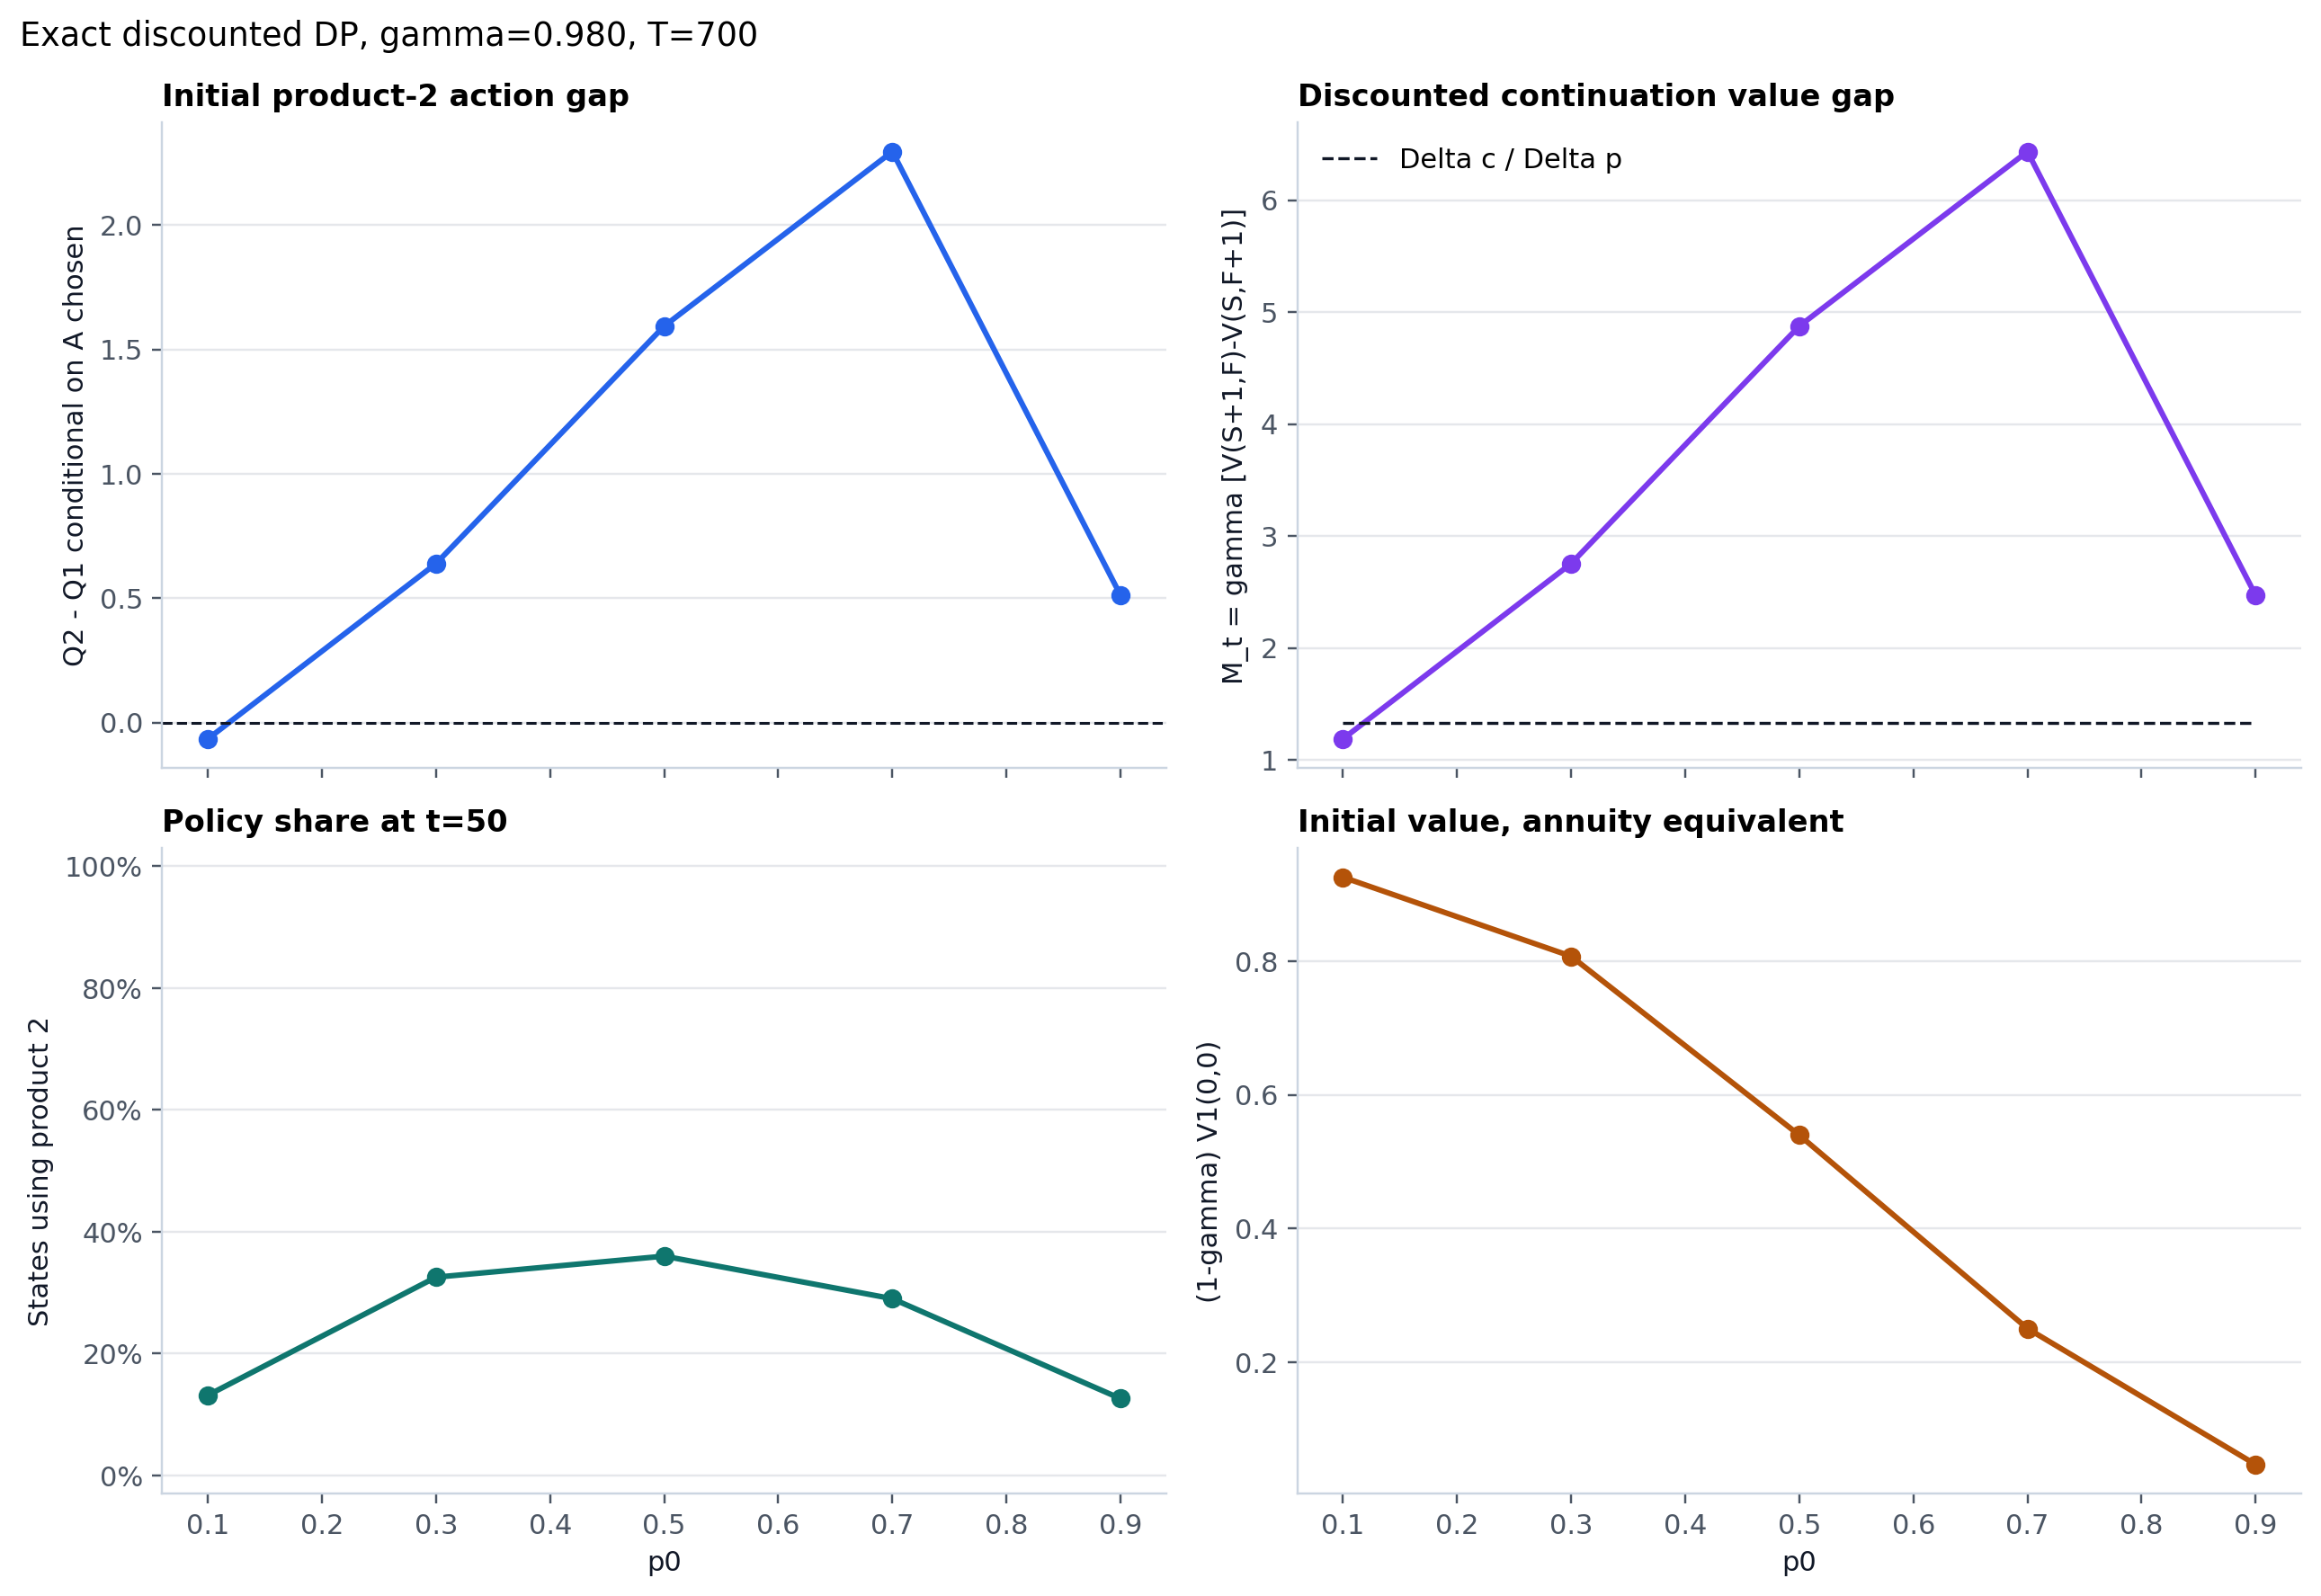
\includegraphics[width=\textwidth]{discounted_initial_summary.png}
    \caption{Summary of Seller A's best response as Seller B's known success probability $p_0$ varies.}
    \label{fig:best-response-by-p0}
\end{figure}

Figure~\ref{fig:best-response-by-p0} summarizes how Seller A's incentives change
with $p_0$.

\begin{itemize}
    \item The top-left panel plots $Q_2(0,0)-Q_1(0,0)$ at the initial state.
    Positive values mean product 2 is optimal at the prior.
    \item The top-right panel reports $M_1(0,0)$ and the $4/3$ threshold.
    \item The bottom-left panel reports the share of reachable states using
    product 2 at the displayed policy period.
    \item The bottom-right panel reports the annuity-equivalent initial value
    $(1-\gamma)V_1(0,0)$.
\end{itemize}

The key pattern is hump-shaped: product 2 is most attractive when Seller A is
neither safely ahead nor hopelessly behind. If $p_0$ is very low, Seller B is
weak, so Seller A can often save cost with product 1. If $p_0$ is very high,
the chance of future demand from A is too low to justify much investment. For
intermediate $p_0$, a success can meaningfully improve future demand, so product
2 is more valuable.

\section{Policy Heatmaps in Count Space}

\begin{figure}[htbp]
    \centering
    
\includegraphics[width=\textwidth]{best_response_policy_heatmaps.png}
    \caption{Optimal product choice over the raw count state space $(S,F)$.}
    \label{fig:count-policy}
\end{figure}

Figure~\ref{fig:count-policy} plots the optimal product for Seller A over the
state space $(S,F)$.

\begin{itemize}
    \item The horizontal axis is the number of observed successes $S$.
    \item The vertical axis is the number of observed failures $F$.
    \item Blue means product 1, the cheap product.
    \item Orange means product 2, the high-quality product.
    \item The blank region is not reachable at the displayed calendar period.
\end{itemize}

The orange regions are states where a success is sufficiently valuable for future
demand. These regions are not simply ``bad reputation'' or ``good reputation''
states. Instead, they tend to occur near reputation margins where the next
outcome can move the user's belief enough to change future choice probabilities.

\section{Policy Over Posterior State Space}

\begin{figure}[htbp]
    \centering
    
\includegraphics[width=\textwidth]{best_response_policy_posterior_state_space.png}
    \caption{Optimal product choice over posterior mean and posterior uncertainty.}
    \label{fig:posterior-policy}
\end{figure}

Figure~\ref{fig:posterior-policy} re-expresses the same policy in posterior
belief coordinates. Each point is still a count state $(S,F)$, but it is plotted
using
\[
    m(S,F) = \mathbb{E}[\theta \mid S,F]
    =
    \frac{1+S}{2+S+F}
\]
on the horizontal axis and the posterior standard deviation on the vertical
axis.

The dashed vertical line is $p_0$. It is the known success probability of Seller
B and therefore the Thompson-sampling comparison threshold. The black dot is the
initial prior $\operatorname{Beta}(1,1)$, which has posterior mean $0.5$ and
standard deviation $\sqrt{1/12}$.

The fan shape is mechanical. As $S+F$ grows, the posterior becomes more precise,
so points move downward. At the same time, different success rates generate
different posterior means, spreading points horizontally. The upper part of the
fan corresponds to low-count, high-uncertainty states; the lower part corresponds
to high-count, precise states.

\section{Value-Difference Diagnostic}

\begin{figure}[htbp]
    \centering
    
\includegraphics[width=\textwidth]{best_response_value_difference_posterior_state_space.png}
    \caption{Diagnostic for the discounted continuation-gap threshold $M_t(S,F)$.}
    \label{fig:value-difference}
\end{figure}

Figure~\ref{fig:value-difference} plots
\[
    M_t(S,F)
    -
    \frac{c_2-c_1}{p_2-p_1}.
\]
Positive values mean product 2 is optimal, while negative values mean product 1
is optimal. This plot is useful because it shows the smooth object behind the
policy rule. The policy plot discretizes states into blue and orange, while
the value-difference plot shows whether those regions come from a coherent
threshold or from numerical noise.

The exact backward induction includes every state reachable at the displayed
period. It does not impose a fixed observation boundary or project histories
back onto a smaller state space.

\section{Horizon Convergence}

The discounted problem is solved at $T=700$, where
$0.98^{700}=7.22\times10^{-7}$. As a direct check, the code re-solves the
problem at $T=850$ and compares the policies over all 1,275 states reachable
at $t=50$.

\begin{figure}[htbp]
    \centering
    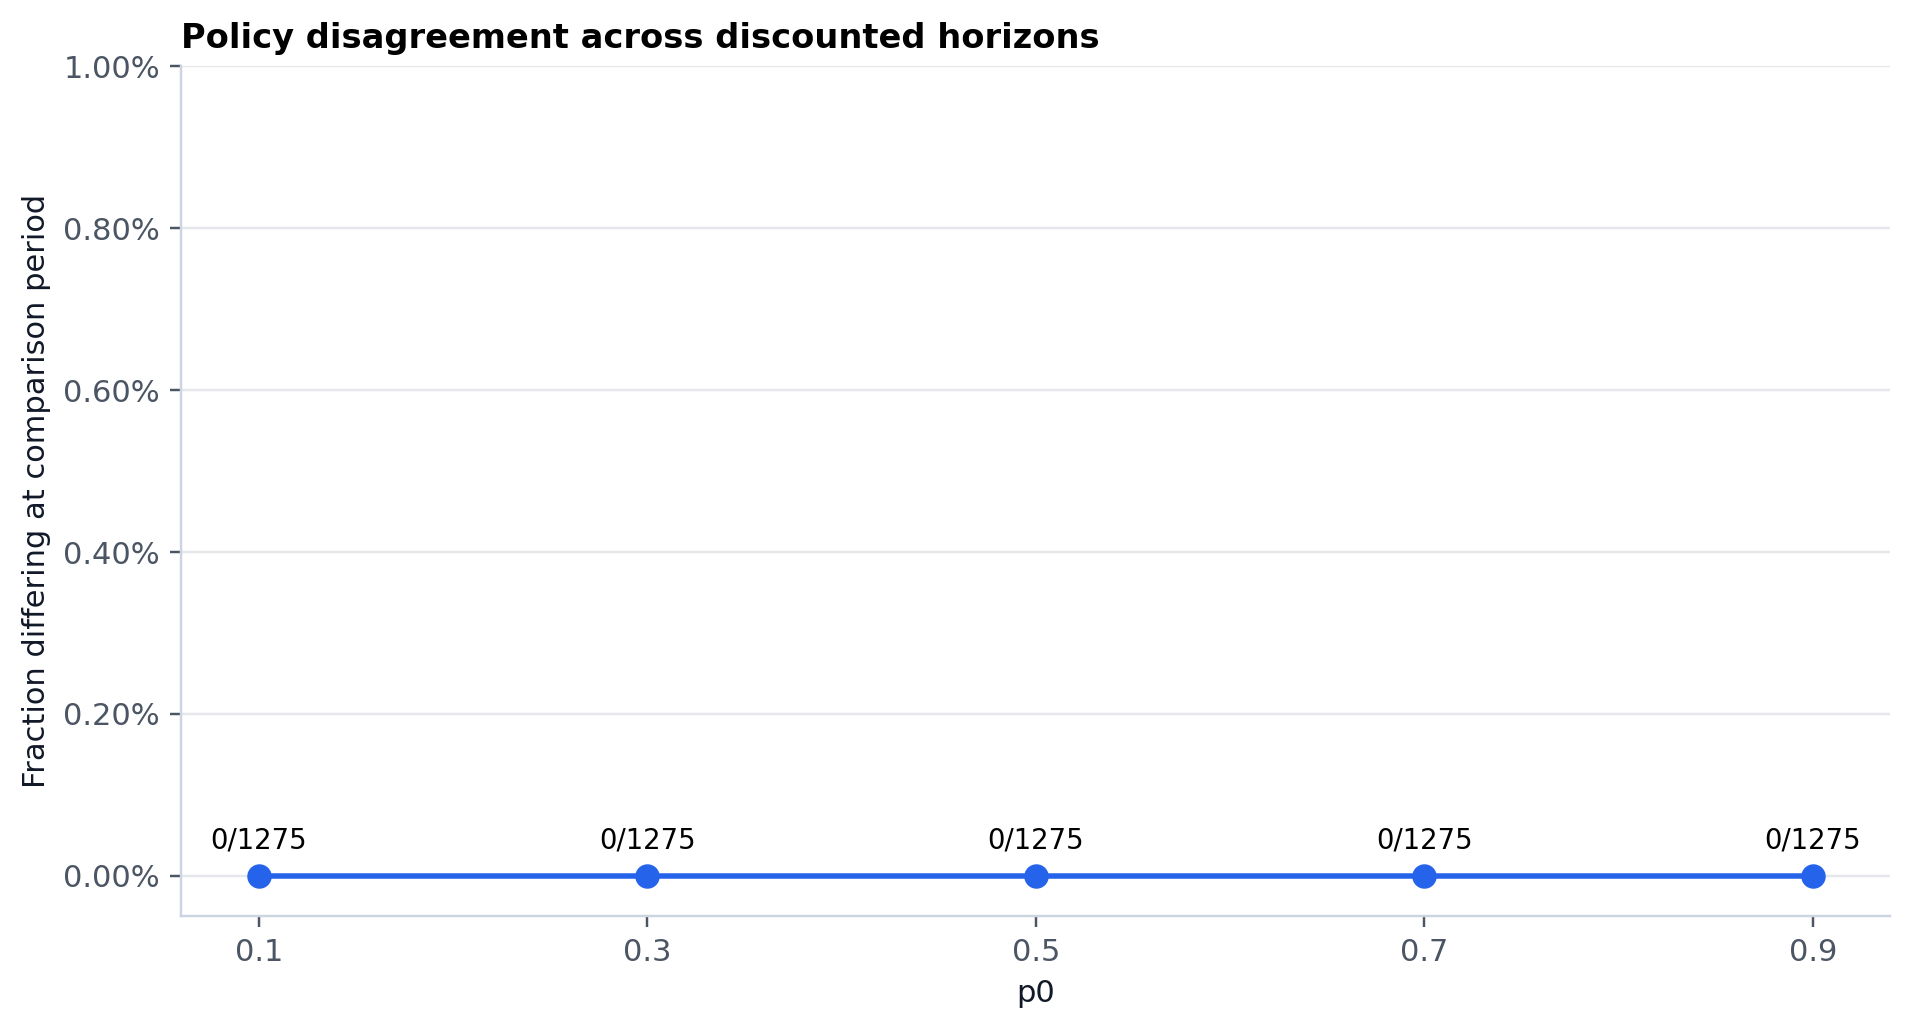
\includegraphics[width=0.82\textwidth]{discounted_horizon_convergence_t50.png}
    \caption{Policy disagreement between $T=700$ and $T=850$ at $t=50$.}
    \label{fig:horizon-convergence}
\end{figure}

\begin{table}[htbp]
\centering
\caption{Policy disagreement between $T=700$ and $T=850$ at $t=50$.}
\label{tab:robustness}
\begin{tabular}{rrr}
\toprule
$p_0$ & States compared & Disagreement \\
\midrule
0.1 & 1,275 & 0\% \\
0.3 & 1,275 & 0\% \\
0.5 & 1,275 & 0\% \\
0.7 & 1,275 & 0\% \\
0.9 & 1,275 & 0\% \\
\bottomrule
\end{tabular}
\end{table}

There are no disagreements for any tested $p_0$. The terminal horizon is
therefore no longer driving the early policy. A direct $p_0=0.5$ comparison
between $T=700$ and $T=2000$ likewise has zero disagreements at $t=50$.

\section{Simulation Path Plot}

\begin{figure}[htbp]
    \centering
    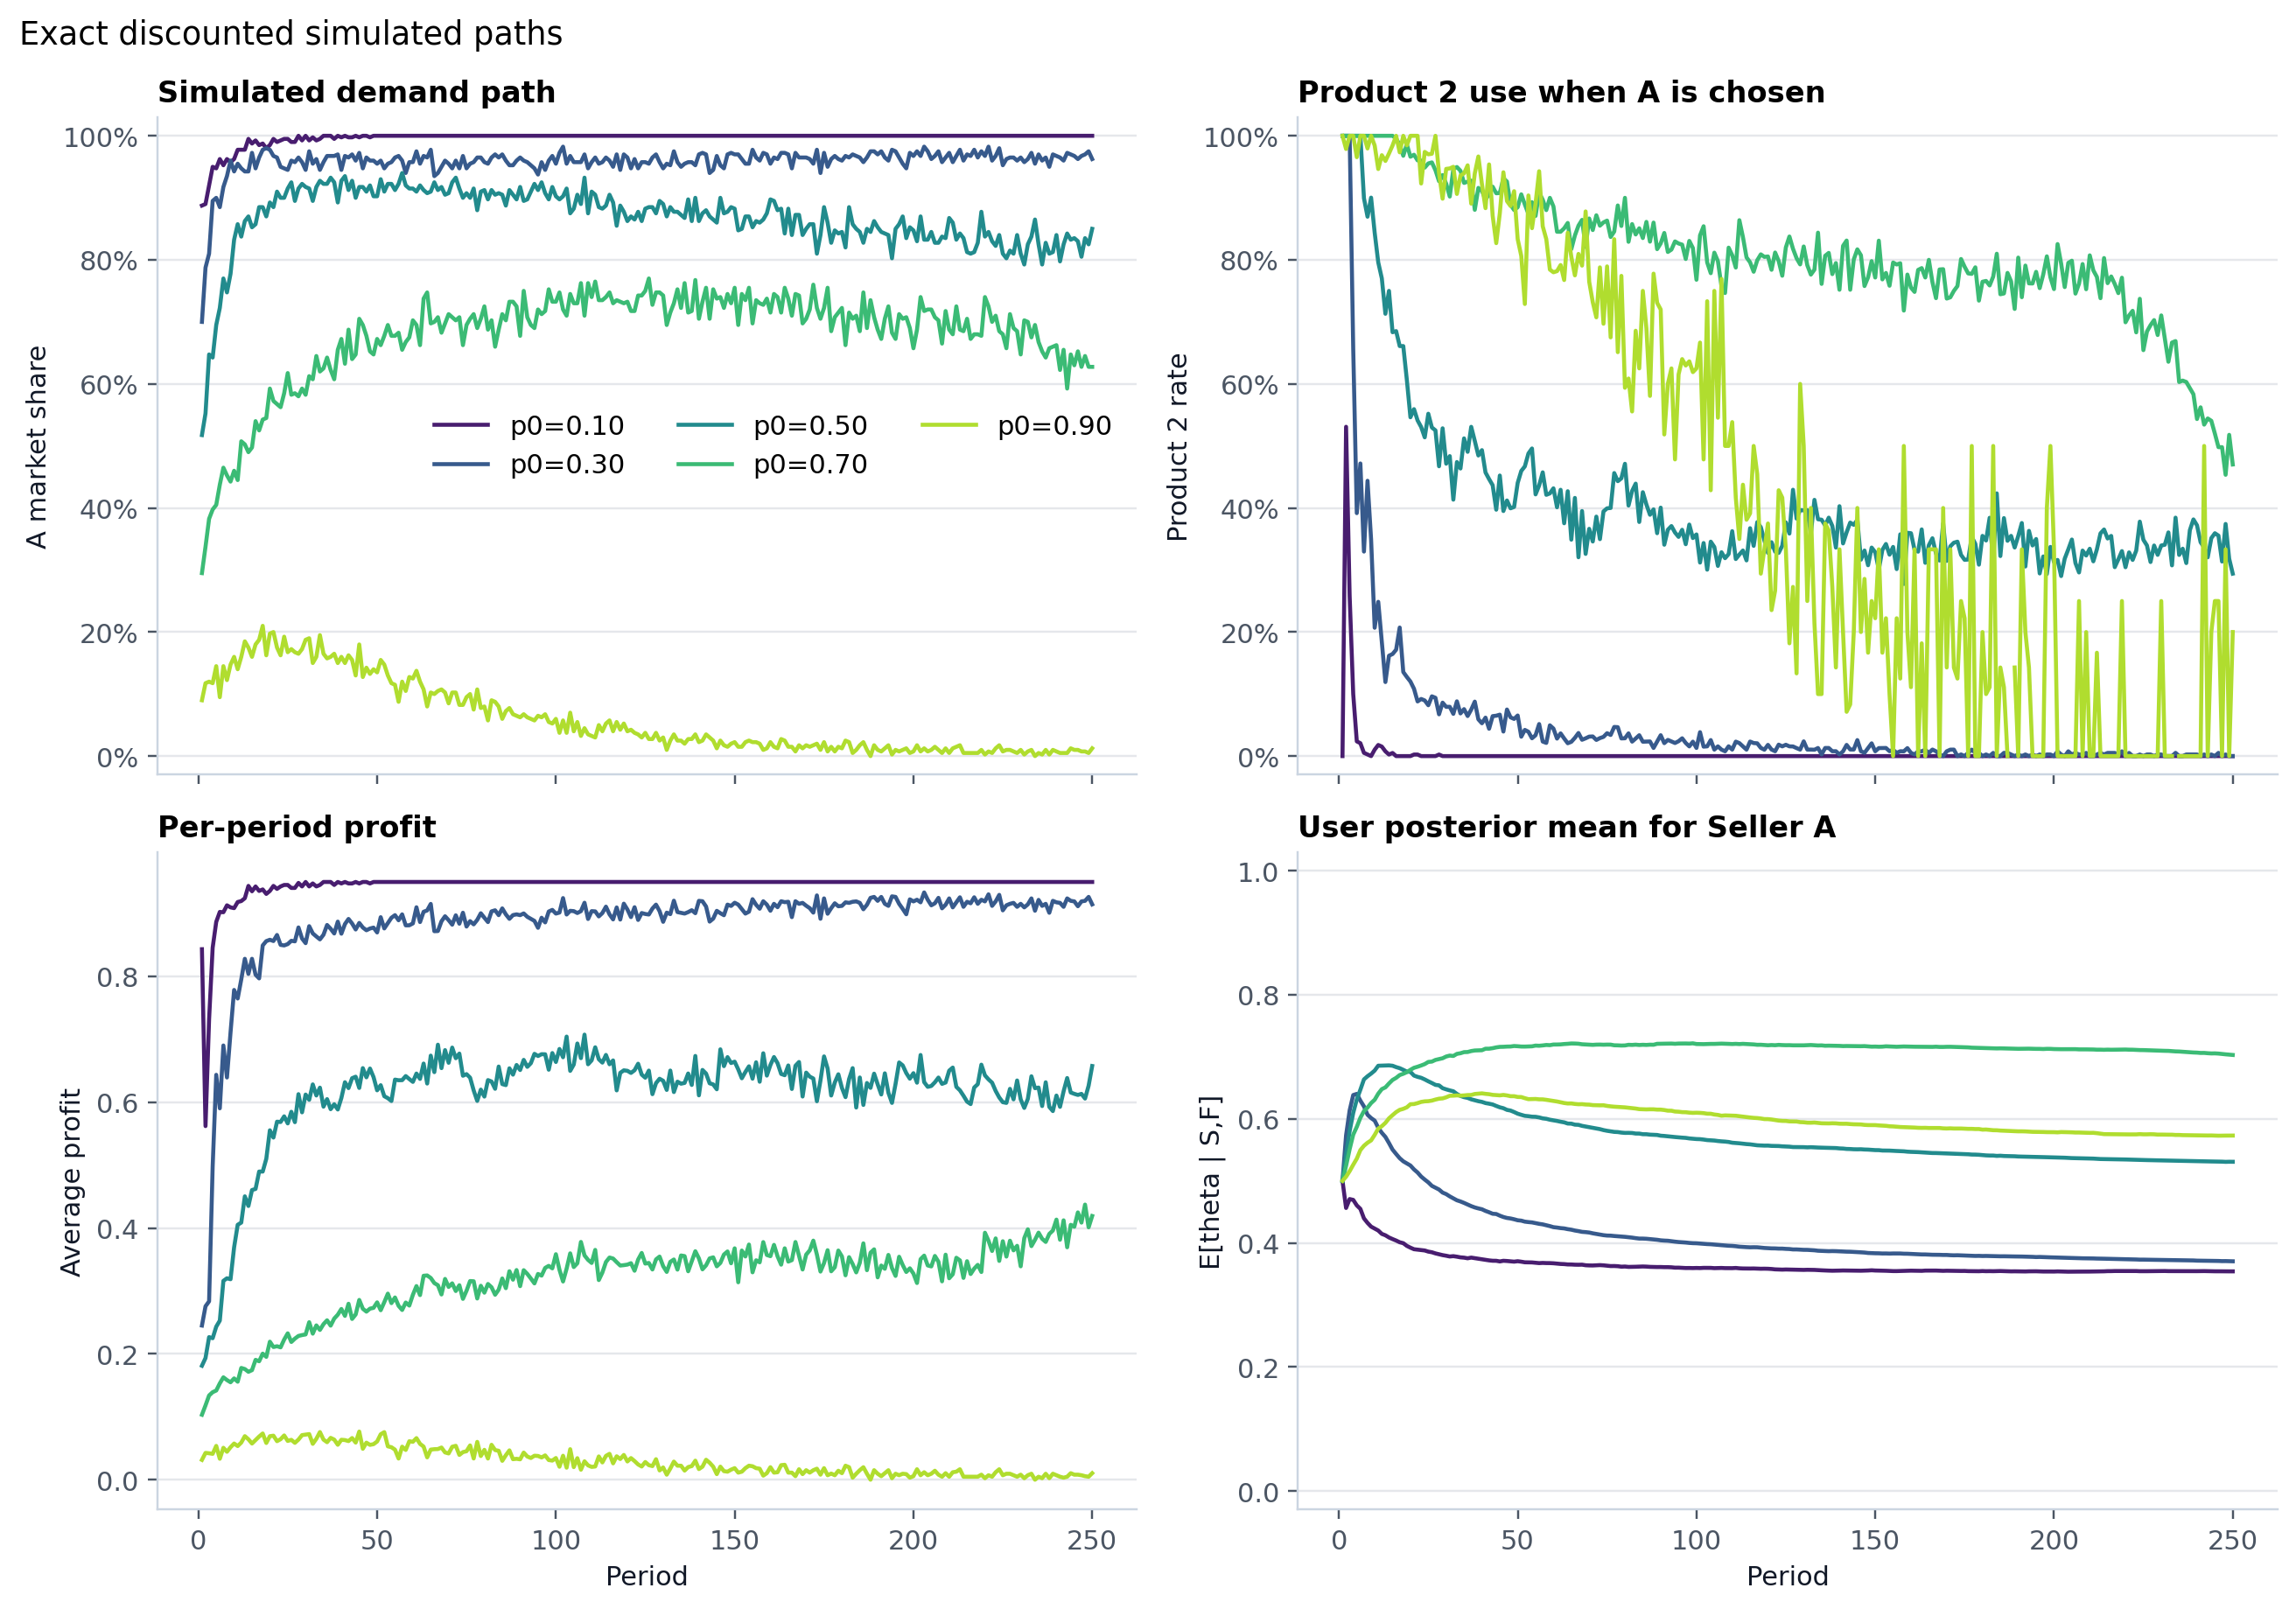
\includegraphics[width=\textwidth]{discounted_simulation_by_period.png}
    \caption{Simulated demand and product 2 usage paths for selected values of $p_0$.}
    \label{fig:simulation-paths}
\end{figure}

Figure~\ref{fig:simulation-paths} shows simulated histories under the solved
best-response policy. The panels track Seller A's market share, product 2 use
conditional on being chosen, per-period profit, and the user's posterior mean.

\begin{figure}[htbp]
    \centering
    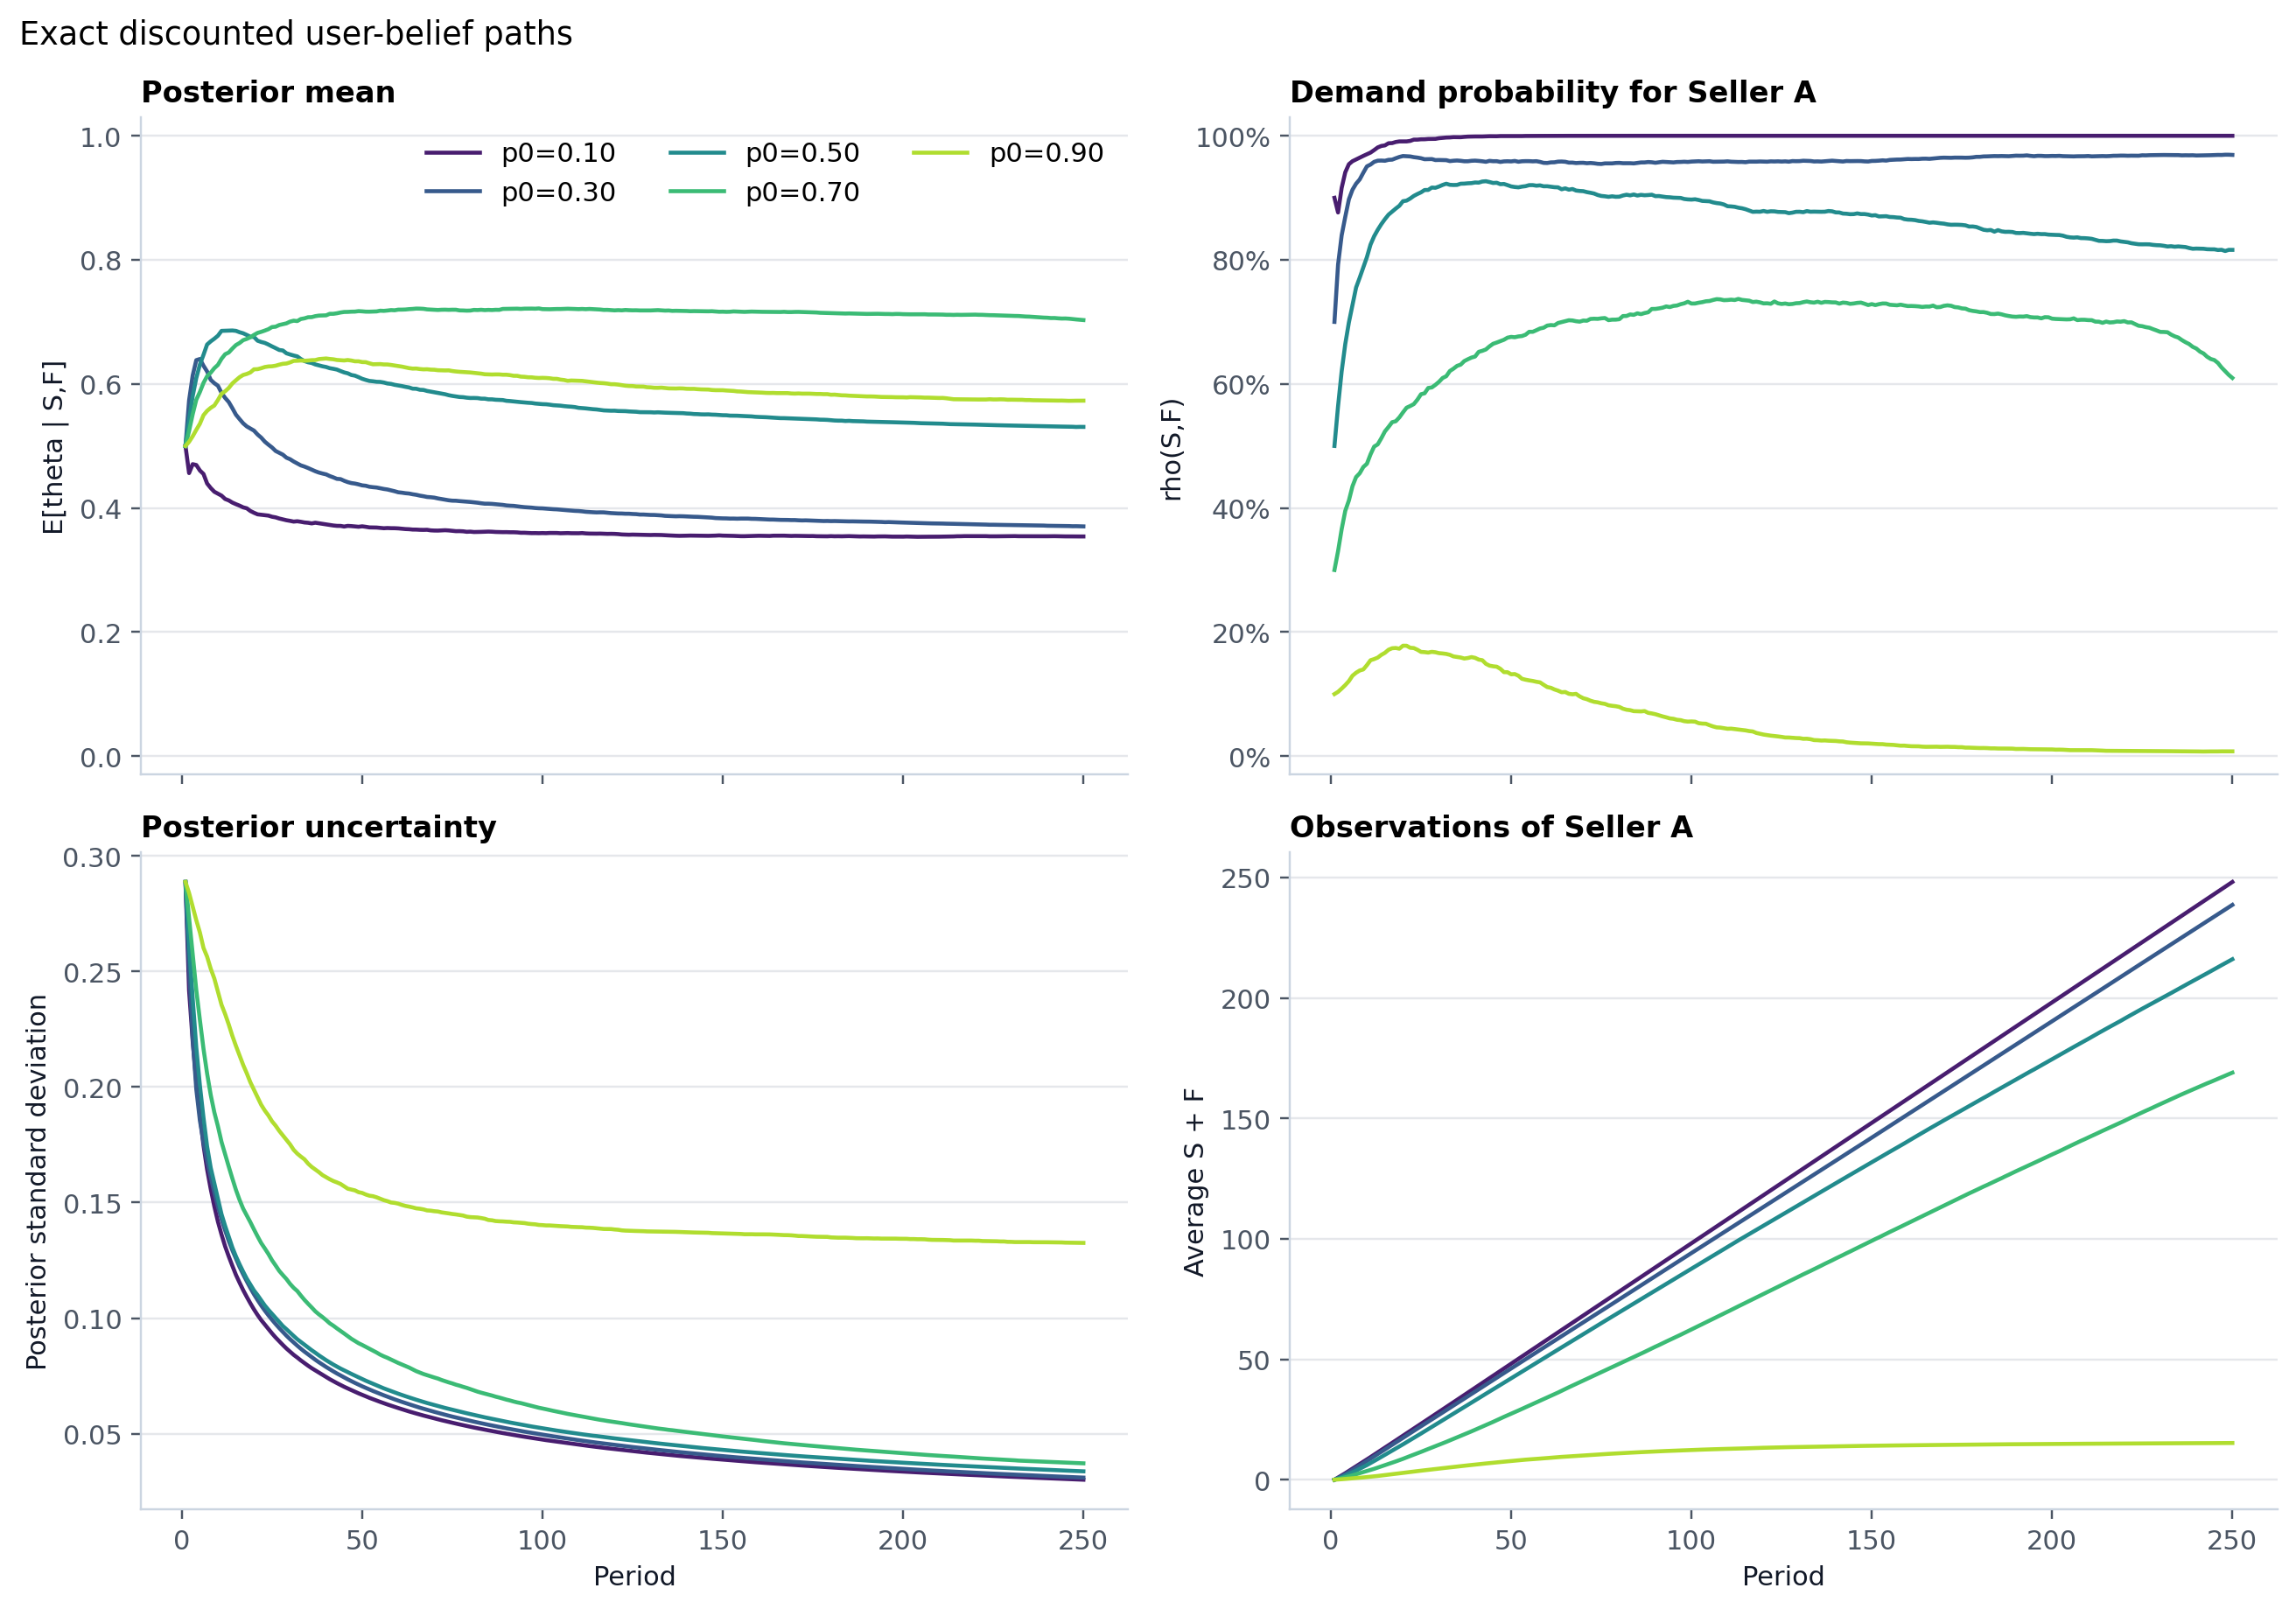
\includegraphics[width=\textwidth]{discounted_user_belief_by_period.png}
    \caption{Simulated user belief paths for selected values of $p_0$.}
    \label{fig:user-belief-paths}
\end{figure}

Figure~\ref{fig:user-belief-paths} shows the user's side of the same simulated
histories. The posterior mean and posterior standard deviation summarize what
the user believes about Seller A before each choice. The demand-probability
panel plots $\rho(S,F)$, the probability that the Thompson-sampling user chooses
Seller A at that period. The observations panel plots the average number of
Seller A outcomes the user has seen.

As $p_0$ increases, Seller A is chosen less often. Conditional on being chosen,
product 2 use tends to rise over the intermediate range because reputation
investment becomes more important. At very high $p_0$, demand is so low that
investment is often not worthwhile.

A fast decline in product 2 use usually means Seller A has already pushed the
user's belief into a safer region. Once the user has many observations of Seller
A, posterior uncertainty falls, and one additional success has a smaller effect
on $\rho(S,F)$. At that point, the costly product 2 has less continuation value,
so the best response can switch back toward product 1 even if demand remains
high.

\end{document}
